\documentclass[a4paper,10pt]{article}
%\documentclass[a4paper,10pt]{scrartcl}

\usepackage[utf8]{inputenc}
\usepackage{tikz}
\usepackage{a4wide}

\title{}
\author{}
\date{}

\pdfinfo{%
  /Title    ()
  /Author   ()
  /Creator  ()
  /Producer ()
  /Subject  ()
  /Keywords ()
}

\begin{document}
\maketitle

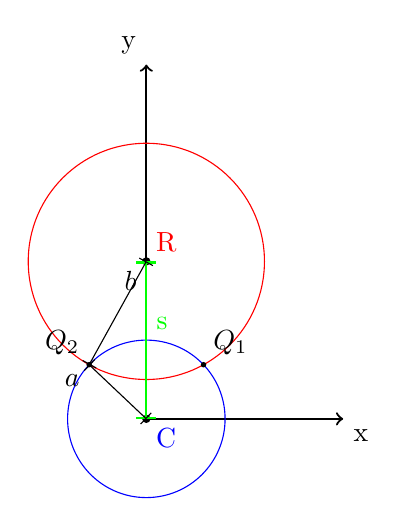
\begin{tikzpicture}
%\draw[step=1cm,gray,very thin] (-3,-3) grid (3,5);
\draw[thick,->] (0,0) -- (2.5,0) node[anchor=north west] {x};
\draw[thick,->] (0,0) -- (0,4.5) node[anchor=south east] {y};
\draw[red] (0,2) circle (1.5cm);
\fill (0,2) circle [radius=1.5pt] node[red,anchor=south west] {R};
\draw[blue] (0,0) circle (1cm);
\fill (0,0) circle [radius=1.5pt] node[blue,anchor=north west] {C};
\draw[green,thick,|-|] (0,0) -- (0,1) node[anchor=south west] {s} -- (0,2);
\fill (0.726184377414,0.6875) circle [radius=1.0pt] node[anchor=south west] {$Q_1$};
\fill (-0.726184377414,0.6875) circle [radius=1.0pt] node[anchor=south east] {$Q_2$};
\draw[|-|] (0,0) -- (-0.726184377414,0.6875) node[anchor=north east] {$a$};
\draw[|-|] (-0.726184377414,0.6875) -- (0,2) node[anchor=north east] {$b$};

\end{tikzpicture}

Berechnung Schnittpunkte:

\begin{eqnarray}
x^2 + y^2 = a^2 \\
(s-x)^2 + y^2 = b^2 \\
x^2 = a^2 - y^2\\
(s-y)^2 + (a^2 - y^2) = b^2\\
s^2 +y^2 - 2ys + a^2 -y^2 -b^2 =0\\
y=\frac{a^2+s^2-b^2}{2s}\\
x_{1,2} =\pm \sqrt{a^2-y}
\end{eqnarray}


Berechnung winkel:\\
\begin{eqnarray}
 s = d \cdot \sin{\frac{\alpha}{2}}\\
\alpha = 2\arcsin{(\frac{s}{d})}
\end{eqnarray}



\end{document}
